\documentclass[10pt,a4paper]{article}
\usepackage[utf8]{inputenc}
\usepackage{amsmath}
\usepackage{amsfonts}
\usepackage{amssymb}
\usepackage{graphicx}
\usepackage{placeins}
\usepackage{wrapfig}
\usepackage{caption}
\usepackage{subcaption}
\usepackage{gensymb}

\begin{document}
\begin{titlepage}
		\centering
		{\scshape\Huge MEEN 368 Design Report: Piston-Crankshaft Assembly}	
		\vspace{1cm}	
		
		{\scshape\Large Texas A\&M University}
		
		{\scshape \large MEEN 368}
		
		\vspace{3 cm}
		
	{\scshape \normalsize Andrew Horn}		
		
		{\scshape \normalsize Rohit Bachani, MoyinOluwa Adejumo, and Gavyn Freeland}

		

		\vfill
		
		{\Large \today}
	\end{titlepage}
\section*{Thermodynamics: Standard Air Analysis}

The engine has 6 cylinders and 3000 c.c. total swept volume. The fuel used will be standard octane gasoline. Intake is taken from the ambient atmosphere.\\
	A Modern Atkinson cycle is chosen in-lieu of the traditional Otto cycle. The Modern Atkinson Cycle is more thermodynamically efficient than the Otto Cycle - reducing fuel and pollution.
	\begin{figure}[h]
		\centering
		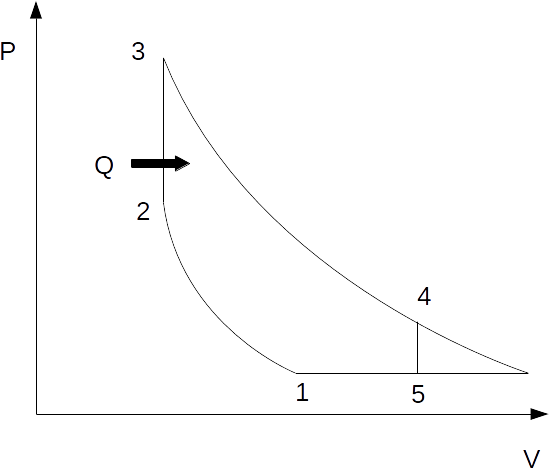
\includegraphics[width=.5\textwidth]{ThermoDiagram.png}
		\caption{PV Diagram of Modern Atkinson Cycle}
		\label{fig:diagram1}
	\end{figure}
	
	Our compression ratio is taken to be 10, a high compression ratio that prevents knocking.
	A lean air to fuel mixture ratio of 29.4 is chosen to ensure complete combustion and limit the pressures. These parameters completely define our thermal cycle.\\ Since the proportion of gasoline is small, and gasoline composed of nonpolar substances, an air standard model is used. The air is not assumed cold - the cold assumption results in far too significant of errors during the combustion process. Gas Tables are used to get air properties.
	\subsection*{Initial Constraints and Constants}
	The compression ratio and air-to-fuel ratio are listed below.
	\begin{align}
		C_R &= \frac{V_1}{V_2} = 10 \\
		M_R &= \frac{m_A}{m_G} = 29.4
	\end{align}
	The total volume swept by the piston is constrained by the total c.c. of the engine.
	\begin{align}
		\frac{3000\ \text{c.c.}}{6} &= V_4-V_2 
	\end{align}
	Point 1 and 5 are at ambient pressure $p_{amb}$, temperature $T_{amb}$, and density $\rho_{amb}$.
	\begin{align}
		p_{amb} &= 101325\ \text{Pa} \\
		T_{amb} &= 288\ \text{K} \\
		\rho_{amb} &= 1.225\ \text{kg}\ \text{m}^{-3}
	\end{align}
	The lower value of the heat of combustion of gasoline referenced from the U.S. EIA.
	\begin{align}
		H_G &= 46.7\ \text{MJ}\ \text{kg}^{-1}
	\end{align}
	\subsection*{State 1}
	This is the start of the compression stroke right after the intake stroke. The air is at ambient conditions, noted in the previous section. The specific volume is calculated and the internal energy taken from an air table.
	\begin{align}
		u_1 &= 205.71\ \text{kJ}\ \text{kg}^{-1}\\
		v_1 &= 0.8163\ \text{m}^3\ \text{kg}^{-1}
	\end{align}
	
	\subsection*{State 1-2}
	The process from state 1 to state 2 is adiabatic compression. The adiabatic compression is assumed isentropic. The compression ratio dictates the final specific volume.
	\begin{align}
		C_R &= \frac{v_1}{v_2}\\
		v_2 &= \frac{v_1}{C_R}\\
		v_2 &= 0.08163\ \text{m}^3\ \text{kg}^{-1}\\
		\rho_2 &= 12.25\ \text{kg}\ \text{m}^{-3}
	\end{align}
	Since it's an isentropic process, the final state can be found from the air table.
	\begin{align}
		T_2 &= 703\ \text{K}\\
		u_2 &= 514.95\ \text{kJ}\ \text{kg}^{-1}
	\end{align}
	\subsection*{State 2-3}
	The process from state 2 to state 3 is an isochoric process with heat added from combustion. The specific heat added is determined from the air to fuel ratio.
	\begin{align}
		m_t &= m_G + m_A = m_G + M_R m_G \\
		Q &= m_G H_G \\
		q &= \frac{Q}{m_t} = \frac{H_G}{1 + M_R}\\
		q &= 1.5362\ \text{MJ}\ \text{kg}^{-1}
	\end{align}
	With no work done on the gas, the final internal energy is given by adding the heat and initial internal energy.
	\begin{align}
		u_3 &= q + u_2\\
		u_3 &= 2051.1\ \text{kJ}\ \text{kg}^{-1}
	\end{align}
	The density is identical, since it's an isochoric process. Additional properties are now derived from the air table.
	\begin{align}
		p_3 &= 8.187\ \text{MPa}\\
		T_3 &= 2385\ \text{K}\\
		\rho_3 &= 12.25\ \text{kg}\ \text{m}^{-3}\\
		p_{3r} &= 4443.2
	\end{align}
	\subsection*{State 3-4}
	This is the expansion stroke - modeled as an adiabatic process. The pressure it expands to is chosen so enough power is produced.
	\begin{align}
		p_4 &= 2.25 p_o = 227.98\ \text{kPa}\\
		p_{4r} &= 123.73
	\end{align}
	Modeling the adiabatic process as isentropic, the relative pressure can be used to find the final properties.
	\begin{align}
		T_4 &= 1022\ \text{K}\\
		u_4 &= 778\ \text{kJ}\ \text{kg}^{-1}\\
		\rho_4 &= 0.777\ \text{kg}\ \text{m}^{-3}
	\end{align}
	\subsection*{Complete Cycle Properties}
	The isentropic processes have no heat transfer - $W = \Delta U$.\\
	The isobaric process has a simple work relation - $W = P \Delta V$.\\
	The specific work is derived from this:
	\begin{align}
		w_{cyc} &= (u_3-u_4) - (u_2-u_1) - p_{amb}(v_4 - v_1) \\
		w_{cyc} &= 1038.3\ \text{kJ}\ \text{kg}^{-1}
	\end{align}
	The total air mass per cylinder is now solved for:
	\begin{align}
		\frac{3000\ \text{c.c.}}{6} &= m_t(v_4-v_2)\\
		m_t &= 414.81E-6\ \text{kg}
	\end{align}
	One cycle is completed per piston for every 2 rotations. The power is given by the mass, specific work, and rotational frequency. The power is evaluated at 8000 R.P.M.
	\begin{align}
		P &= 6 m_t w_{cyc} \frac{f}{2}\\
		P &= 172.28\ \text{kW}= 231.0\ \text{hp}\\
		\eta &= \frac{w_{cyc}}{q}= 67.6 \%
	\end{align}
	Real world efficiencies are expected to be far lower.
	\newpage
	
	\section*{System Dynamics}
	
	\begin{wrapfigure}{R}{.23\textwidth}
		\centering
		\caption*{Crank Linkage}
		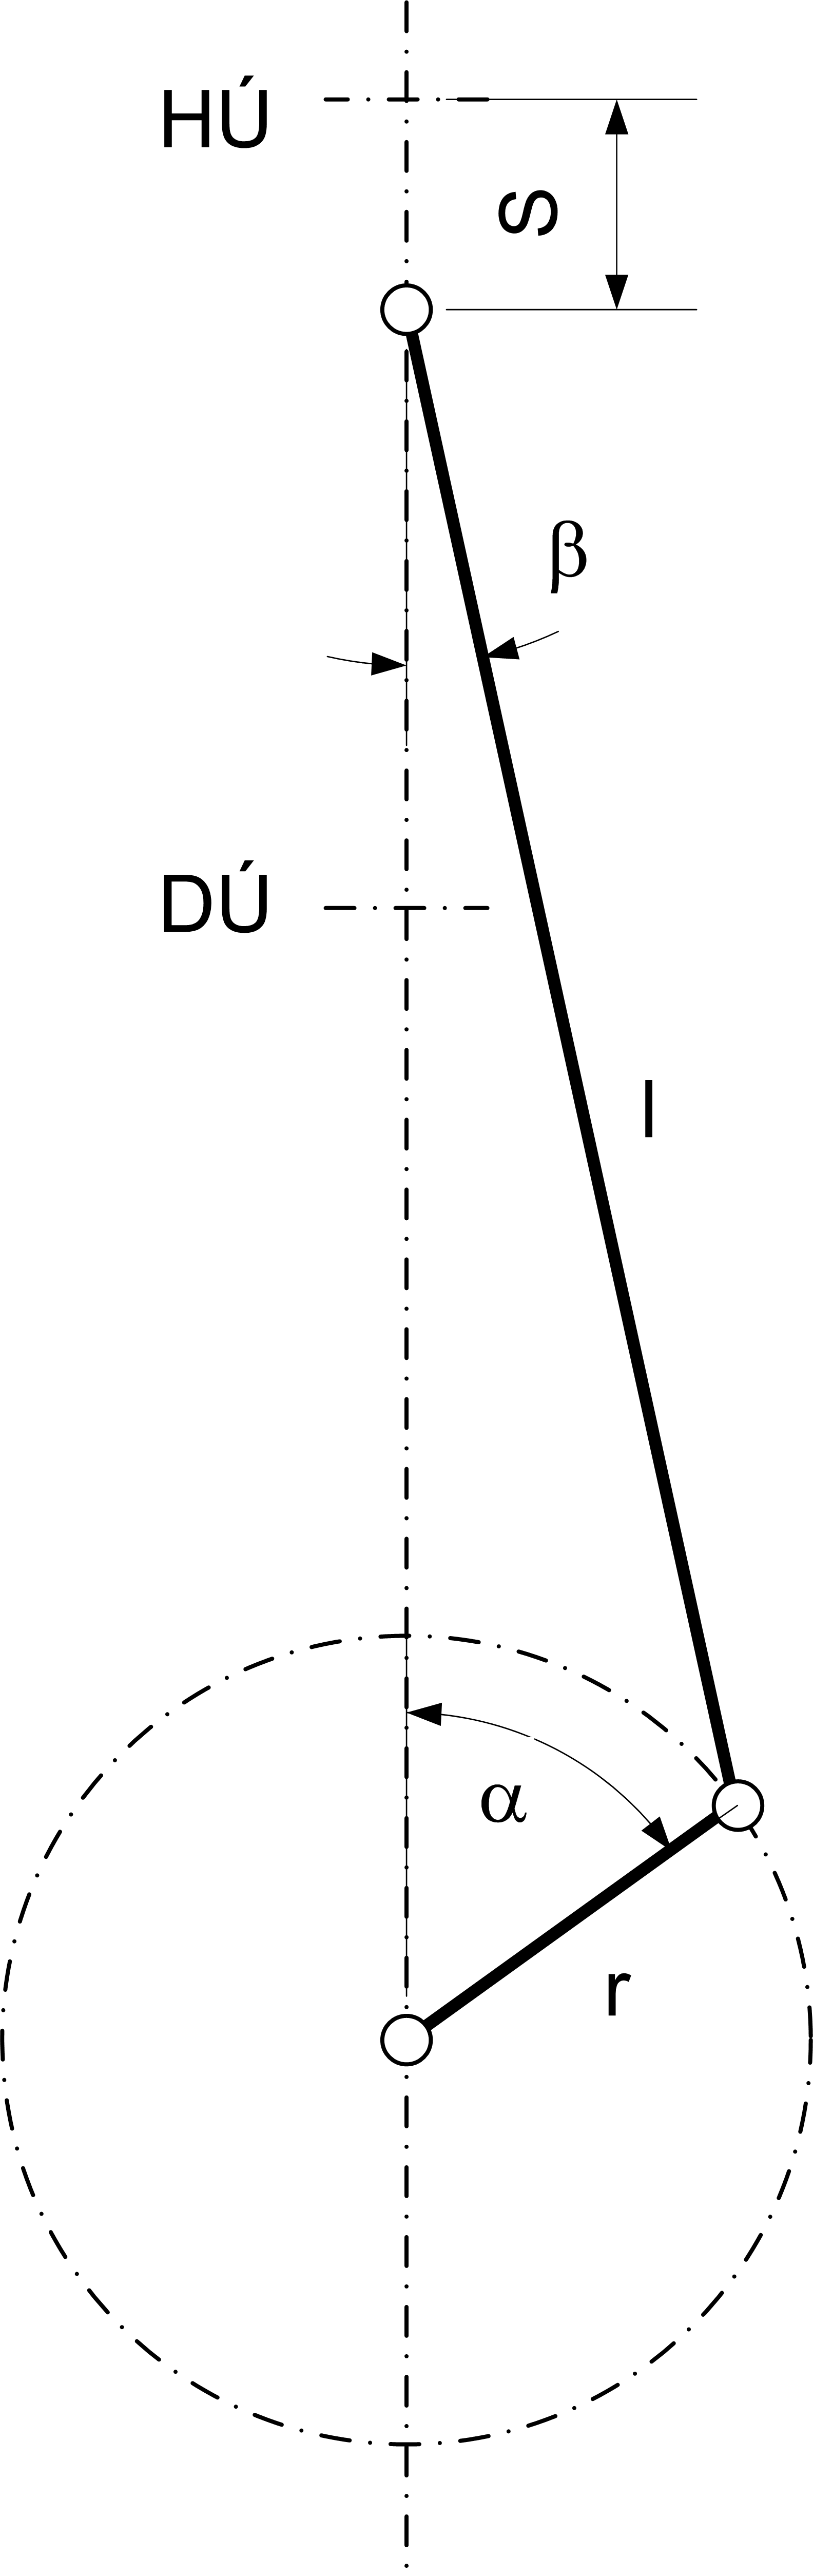
\includegraphics[width=.17\textwidth]{CrankDiagram.png}
		\label{fig:diagram2}
		\caption*{{\tiny \textit{Used with permission from WikiMedia Foundation}}}
		
	\end{wrapfigure}
	To derive the piston forces, first the linear kinematics of the piston head needs to derived with respect to $\alpha = \omega t$, where $\theta = 0$ is TDC and $x$ is the distance below TDC. \\
	The crankshaft radius is $r$ and the connecting rod length is $l_CR$. The height from the crank center is given by $r \cos (\alpha) = r \cos (\omega t)$. The height from the connecting rod is derived from noting the triangles formed by the crankshaft and connecting rod share an edge. $l_{CR} \cos (\beta)$ is solved for in terms of $\alpha$.
	\begin{align}
		r \sin(\alpha) &= l_{CR} \sin (\beta)\\
		\frac{r}{l_{CR}}\sin(\alpha) &= \sin (\beta)\\
		\cos(\beta) &= \sqrt{1 - \Big( \frac{r}{l_{CR}}\sin(\alpha) \Big)^2}\\
		l_{CR} \cos (\beta) &= \sqrt{l_{CR}^2 - (r \sin (\alpha))^2}
	\end{align}
	The position is given by $r \cos (\omega t) + l_{CR} \cos (\beta)$. The equation is adjusted such that $x(0)=0$ and downwards is positive. The derivatives are derived with a symbolic algebra program. These dynamic equations are used to later derive the forces on the piston and crankshaft.\\
\begin{align}
	x(t ) &= (r + l_{CR}) - \Big(r \cos (\omega t)  + \sqrt{l_{\text{CR}}^2 - r^2 \sin^2 (\omega t )} \Big)\\
	v(t ) &=  \frac{\omega r^{2} \sin{\left (\omega t \right )} \cos{\left (\omega t \right )}}{\sqrt{l_{CR}^{2} - r^{2} \sin^{2}{\left (\omega t \right )}}} + \omega r \sin{\left (\omega t \right )}\\
	a (t) &=  \frac{\omega^{2} r^{4} \sin^{2}{\left (\omega t \right )} \cos^{2}{\left (\omega t \right )}}{\left(l_{CR}^{2} - r^{2} \sin^{2}{\left (\omega t \right )}\right)^{\frac{3}{2}}} - \frac{\omega^{2} r^{2} \sin^{2}{\left (\omega t \right )}}{\sqrt{l_{CR}^{2} - r^{2} \sin^{2}{\left (\omega t \right )}}}\nonumber \\
	&  \qquad \qquad + \frac{\omega^{2} r^{2} \cos^{2}{\left (\omega t \right )}}{\sqrt{l_{CR}^{2} - r^{2} \sin^{2}{\left (\omega t \right )}}} + \omega^{2} r \cos{\left (\omega t \right )}
\end{align}
\newpage

\section*{Forces}
To get the force of the piston, pressures equations are needed. The pressure of the expansion and compression strokes relative to piston position are approximated with the adiabatic relation $P V^{\gamma} = c$.
The pressure of the intake and compression strokes are derived using mass flow rates and Bernoulli's equation.\\
At the TDC, the height of the air column is given by $z = \frac{V_{\text{comp}}}{A_C}$, where $A_C$ is the cross sectional area of the chamber and $V_{\text{comp}}$ is the air volume at compression.\\ Thus air volume at any point of piston movement is $V(t) = A_C (x(t)+z)$.
\subsection*{Compression Stroke}
The compression stroke is derived using adiabatic relations $P V^{\gamma} = c$.
\begin{align}
	P_{\text{amb}} V_1^{\gamma} &= P(t) V(t)^{\gamma}\\
	P_{\text{Compression}}(t) &= P_{\text{amb}} \Big( \frac{V_1}{A_C (x(t)+z)} \Big)^{\gamma}
\end{align}
\subsection*{Expansion Stroke} 
The expansion stroke is derived the same way.
\begin{align}
	P_{4} V_{\text{comp}}^{\gamma} &= P(t) V(t)^{\gamma}\\
	P_{\text{Expansion}}(t) &= P_{4} \Big( \frac{V_{\text{comp}}}{A_C (x(t)+z)} \Big)^{\gamma}
\end{align}
\subsection*{Intake/Exhaust Strokes}
The pressure difference in the intake/exhaust strokes is derived using bernoulli equations. A 0 air velocity in the piston chamber is assumed. For simplicity, the density is assumed constant. The pressure difference needed to balance the air flow rates is found. \\ Let $A_I$ be the cross sectional area of the intake valve.
\begin{align}
	Q &= A_I v_a \rho_{\text{amb}} = A_C v(t)\rho_{\text{amb}}\\
	v &= \frac{A_C v(t)}{A_I}\\
	\Delta P &= \frac{1}{2} \rho_{\text{amb}} v^2 \\
	\Delta P &= \frac{1}{2} \rho_{\text{amb}} \Big( \frac{A_C v(t)}{A_I} \Big)^2
\end{align}
\subsection*{Gas Forces}
The force on the piston from the gasses is a function of pressure and chamber area. Compressive forces are taken to be positive. \\
 Simply, $$F_{\text{Gasses}} = A_C (P(t) - P_{\text{amb}})$$\\
 The total gas force function is given by a piecewise function. Let $\theta_c$ is the angle such that $x(t) = 9z$ and $v(t) < 0$. Then  $F_{\text{Gas}}$ is
\begin{align}
F_{\text{Gas}}(t) &=
\begin{cases}
A_C \Big(P_{4} \Big( \frac{V_4}{A_C (x(t)+z)} \Big)^{\gamma} - P_{\text{amb}}\Big) - (m_P+m_{CR})a(t) & 0^\circ \leq \omega t \mod 720^\circ \leq 180^\circ \\
A_C \frac{1}{2} \rho_{\text{amb}} \Big( \frac{A_C v(t)}{A_I} \Big)^2 - (m_P+m_{CR})a(t) & 180^\circ < \omega t \mod 720^\circ \leq 360^\circ \\
- A_C \frac{1}{2} \rho_{\text{amb}} \Big( \frac{A_C v(t)}{A_I} \Big)^2 - (m_P+m_{CR})a(t) & 360^\circ < \omega t \mod 720^\circ \leq 540^\circ \\
A_C \frac{1}{2} \rho_{\text{amb}} \Big( \frac{A_C v(t)}{A_I} \Big)^2 - (m_P+m_{CR})a(t) & 540^\circ < \omega t \mod 720^\circ \leq 360^\circ + \theta_c \\
A_C \Big( P_{\text{amb}} \Big( \frac{V_1}{A_C (x(t)+z)} \Big)^{\gamma}- P_{\text{amb}}\Big) - (m_P+m_{CR})a(t) & 360^\circ + \theta_c < \omega t \mod 720^\circ < 720^\circ \\
\end{cases}
\end{align}
\subsection*{Acceleration Forces}
Additionally there exists a body force present due to the acceleration of the piston head. Since compressive forces are positive, the acceleration term is inverted. Assuming $l_{CR} >> r$, the acceleration of the connecting rod is assumed equivalent to piston acceleration. For the forces on the piston, only the piston mass matters. For the forces on the crankshaft, both the piston mass $m_p$ and connecting rod mass $m_{CR}$ are needed.
$$F_{\text{accel}}(t) = - m_p a(t)$$
The total force on the piston is from both the acceleration terms and gas force terms.
\begin{align}
\vec{F}(t) &= \big \langle -F(t)\ \hat{i},\ F(t) \frac{r \sin(\omega t)}{\sqrt{l^2 - r^2 \sin^2(\omega t)}}  \hat{j} \big \rangle\\
\vec{F}_n(t) &= \vec{F}(t + 120 \degree (n-1)\omega^{-1})
\end{align}

\end{document}